\section{A MAC Layer in \mbox{Mote Runner}}
\begin{frame}[fragile]
  \frametitle{Design strategy}
  \begin{itemize}
  	\item Beacon enabled, A-TDM with CSMA/CA
    \item Mac class behaviours:
    \begin{itemize}
      \item Coordinator -> Sends beacons and handles request and data frames from motes
      \item Unassociated -> Tries to associate with a Coordinator
      \item Associated -> Sends data from upper layer and receives data from Coordinator
    \end{itemize}
    \item Focus on flexibility:
    \begin{itemize}
    	\item State changes have to be ruled by Mac class through events
    	\item Mac should handle more than one state -> Mac - entities
    	\begin{itemize}
	  \item e.g.: a single mote acting as Coordinator and Associated
    	\end{itemize}
    \end{itemize}
  \end{itemize}
\end{frame}

\begin{frame}[fragile]
  \frametitle{The network's concept}
  \begin{figure}
    \centering
    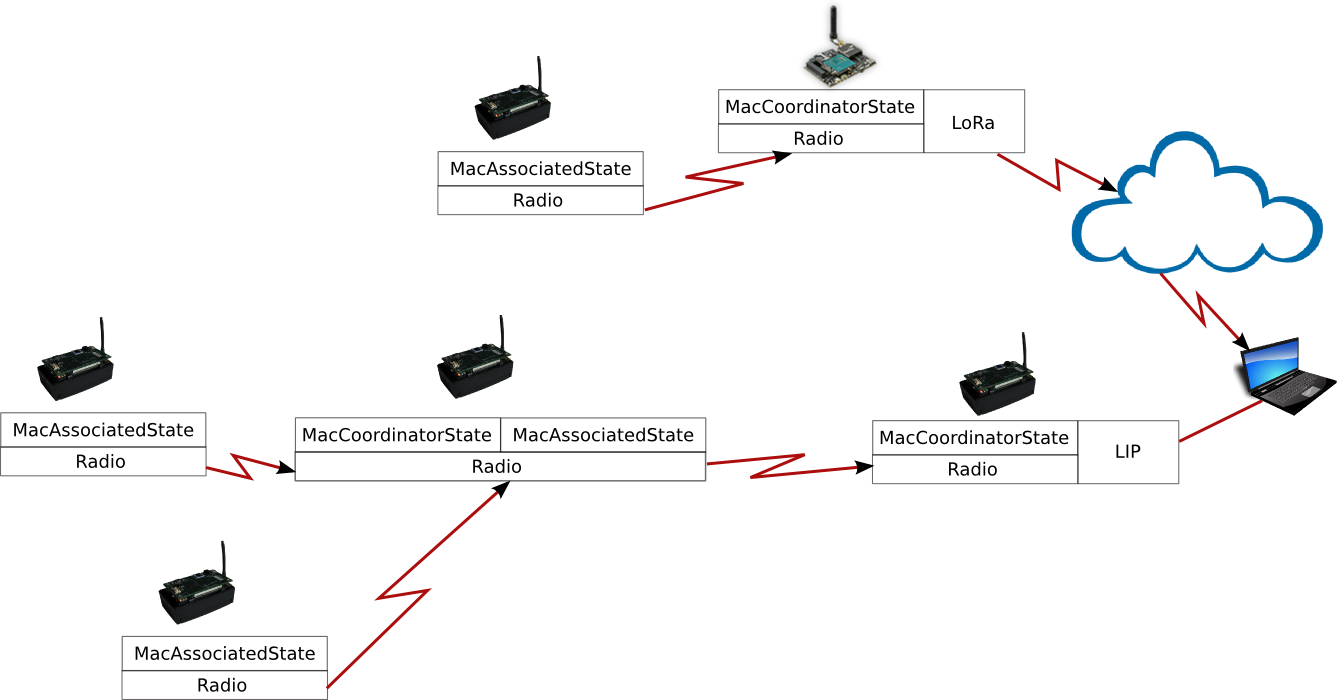
\includegraphics[width=\textwidth]{img/MAClan.png}
  \end{figure}
\end{frame}

\begin{frame}[fragile]
  \frametitle{About the network}
  \begin{itemize}
    \item Motes are subdivided into PANs
    \begin{itemize}
    	\item Every PAN has a PAN ID
    	\item Every mote has a unique short address (SADDR) inside the PAN
    \end{itemize}
    \item To obtain the SADDR the mote must associate with the PAN coordinator
    \item To grant communication between motes synchronization is crucial
    \begin{itemize}
      \item Beacon + Superframe
    \end{itemize}
    \item The adopted procedures follow 802.15.4 standard
  \end{itemize}
\end{frame}

\begin{frame}[fragile]
  \frametitle{Association}
  \begin{figure}
    \centering
    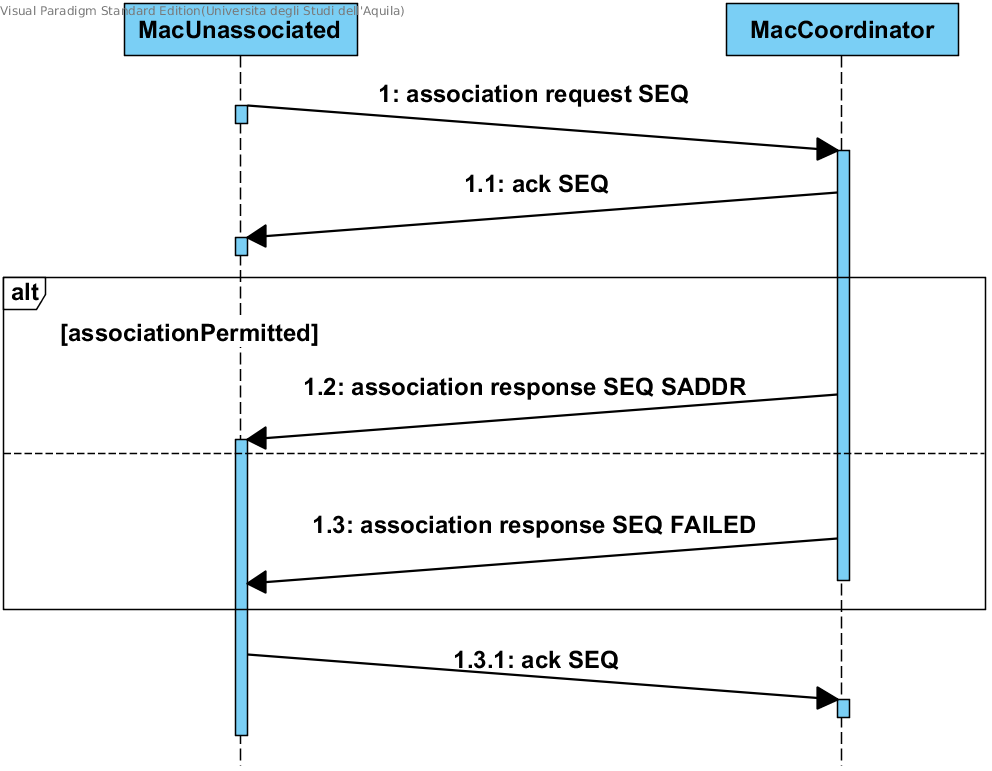
\includegraphics[width=.8\textwidth]{img/Association.png}
  \end{figure}
\end{frame}

\begin{frame}[fragile]
  \frametitle{Data indirect}
%  \vspace{-2.7em}
  \begin{figure}
    \centering
    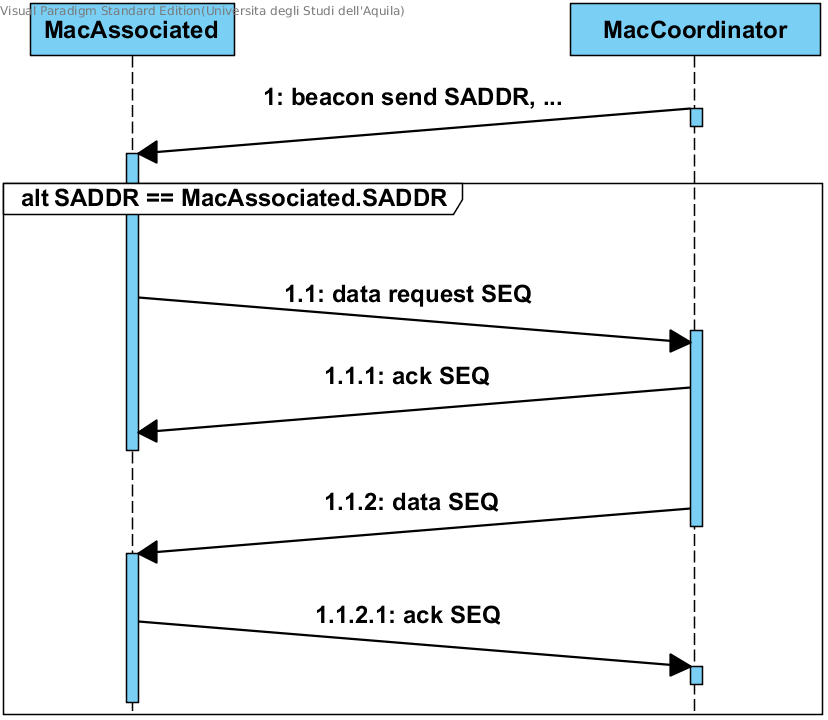
\includegraphics[width=.7\textwidth]{img/DataRequest.png}
  \end{figure}
\end{frame}

\begin{frame}[fragile]
  \frametitle{Timing with beacon}
  \begin{itemize}
    \item Grants synchronization between mote and coordinator
    \item Realized with a timer and scheduled events
  \end{itemize}
  \begin{figure}
    \centering
    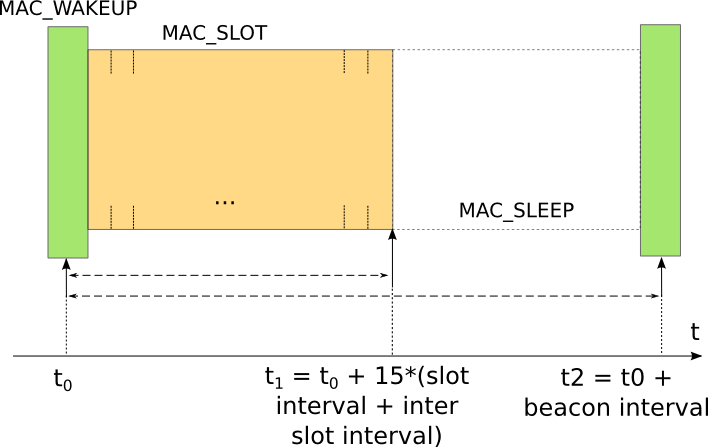
\includegraphics[width=.7\textwidth]{img/MAC_STATES.png}
  \end{figure}
\end{frame}

\begin{frame}[fragile]
  \frametitle{Beacon}
  \vspace{-2em}
  \begin{columns}
    \begin{column}{.58\linewidth}
      \begin{itemize}
	\item Superframe Specification:
	\begin{itemize}
	  \item Beacon Order -> BO
	  \item Superframe Order -> SO
	  \item Association permitted
	\end{itemize}
      \end{itemize}
    \end{column}
    \hfill
    \begin{column}{.4\linewidth}
      \begin{figure}
	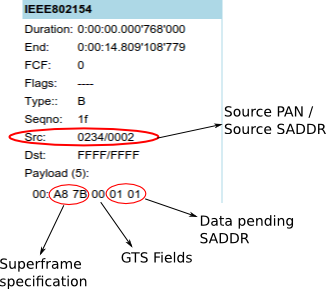
\includegraphics[width=\textwidth]{img/beacon.png}
      \end{figure}
    \end{column}
  \end{columns}
  \vspace{1em}
  $$\text{Beacon Interval} = \frac{60sym \cdot n.Slot \cdot
2^{BO}}{20\text{kbps}}$$
  $$\text{Superframe Duration} = \frac{60sym \cdot n.Slot \cdot
2^{SO}}{20\text{kbps}}$$
\end{frame}


\begin{frame}[fragile]
  \frametitle{Mac Coordinator Behaviour}
  \vspace{-2.7em}
  \begin{figure}
    \centering
    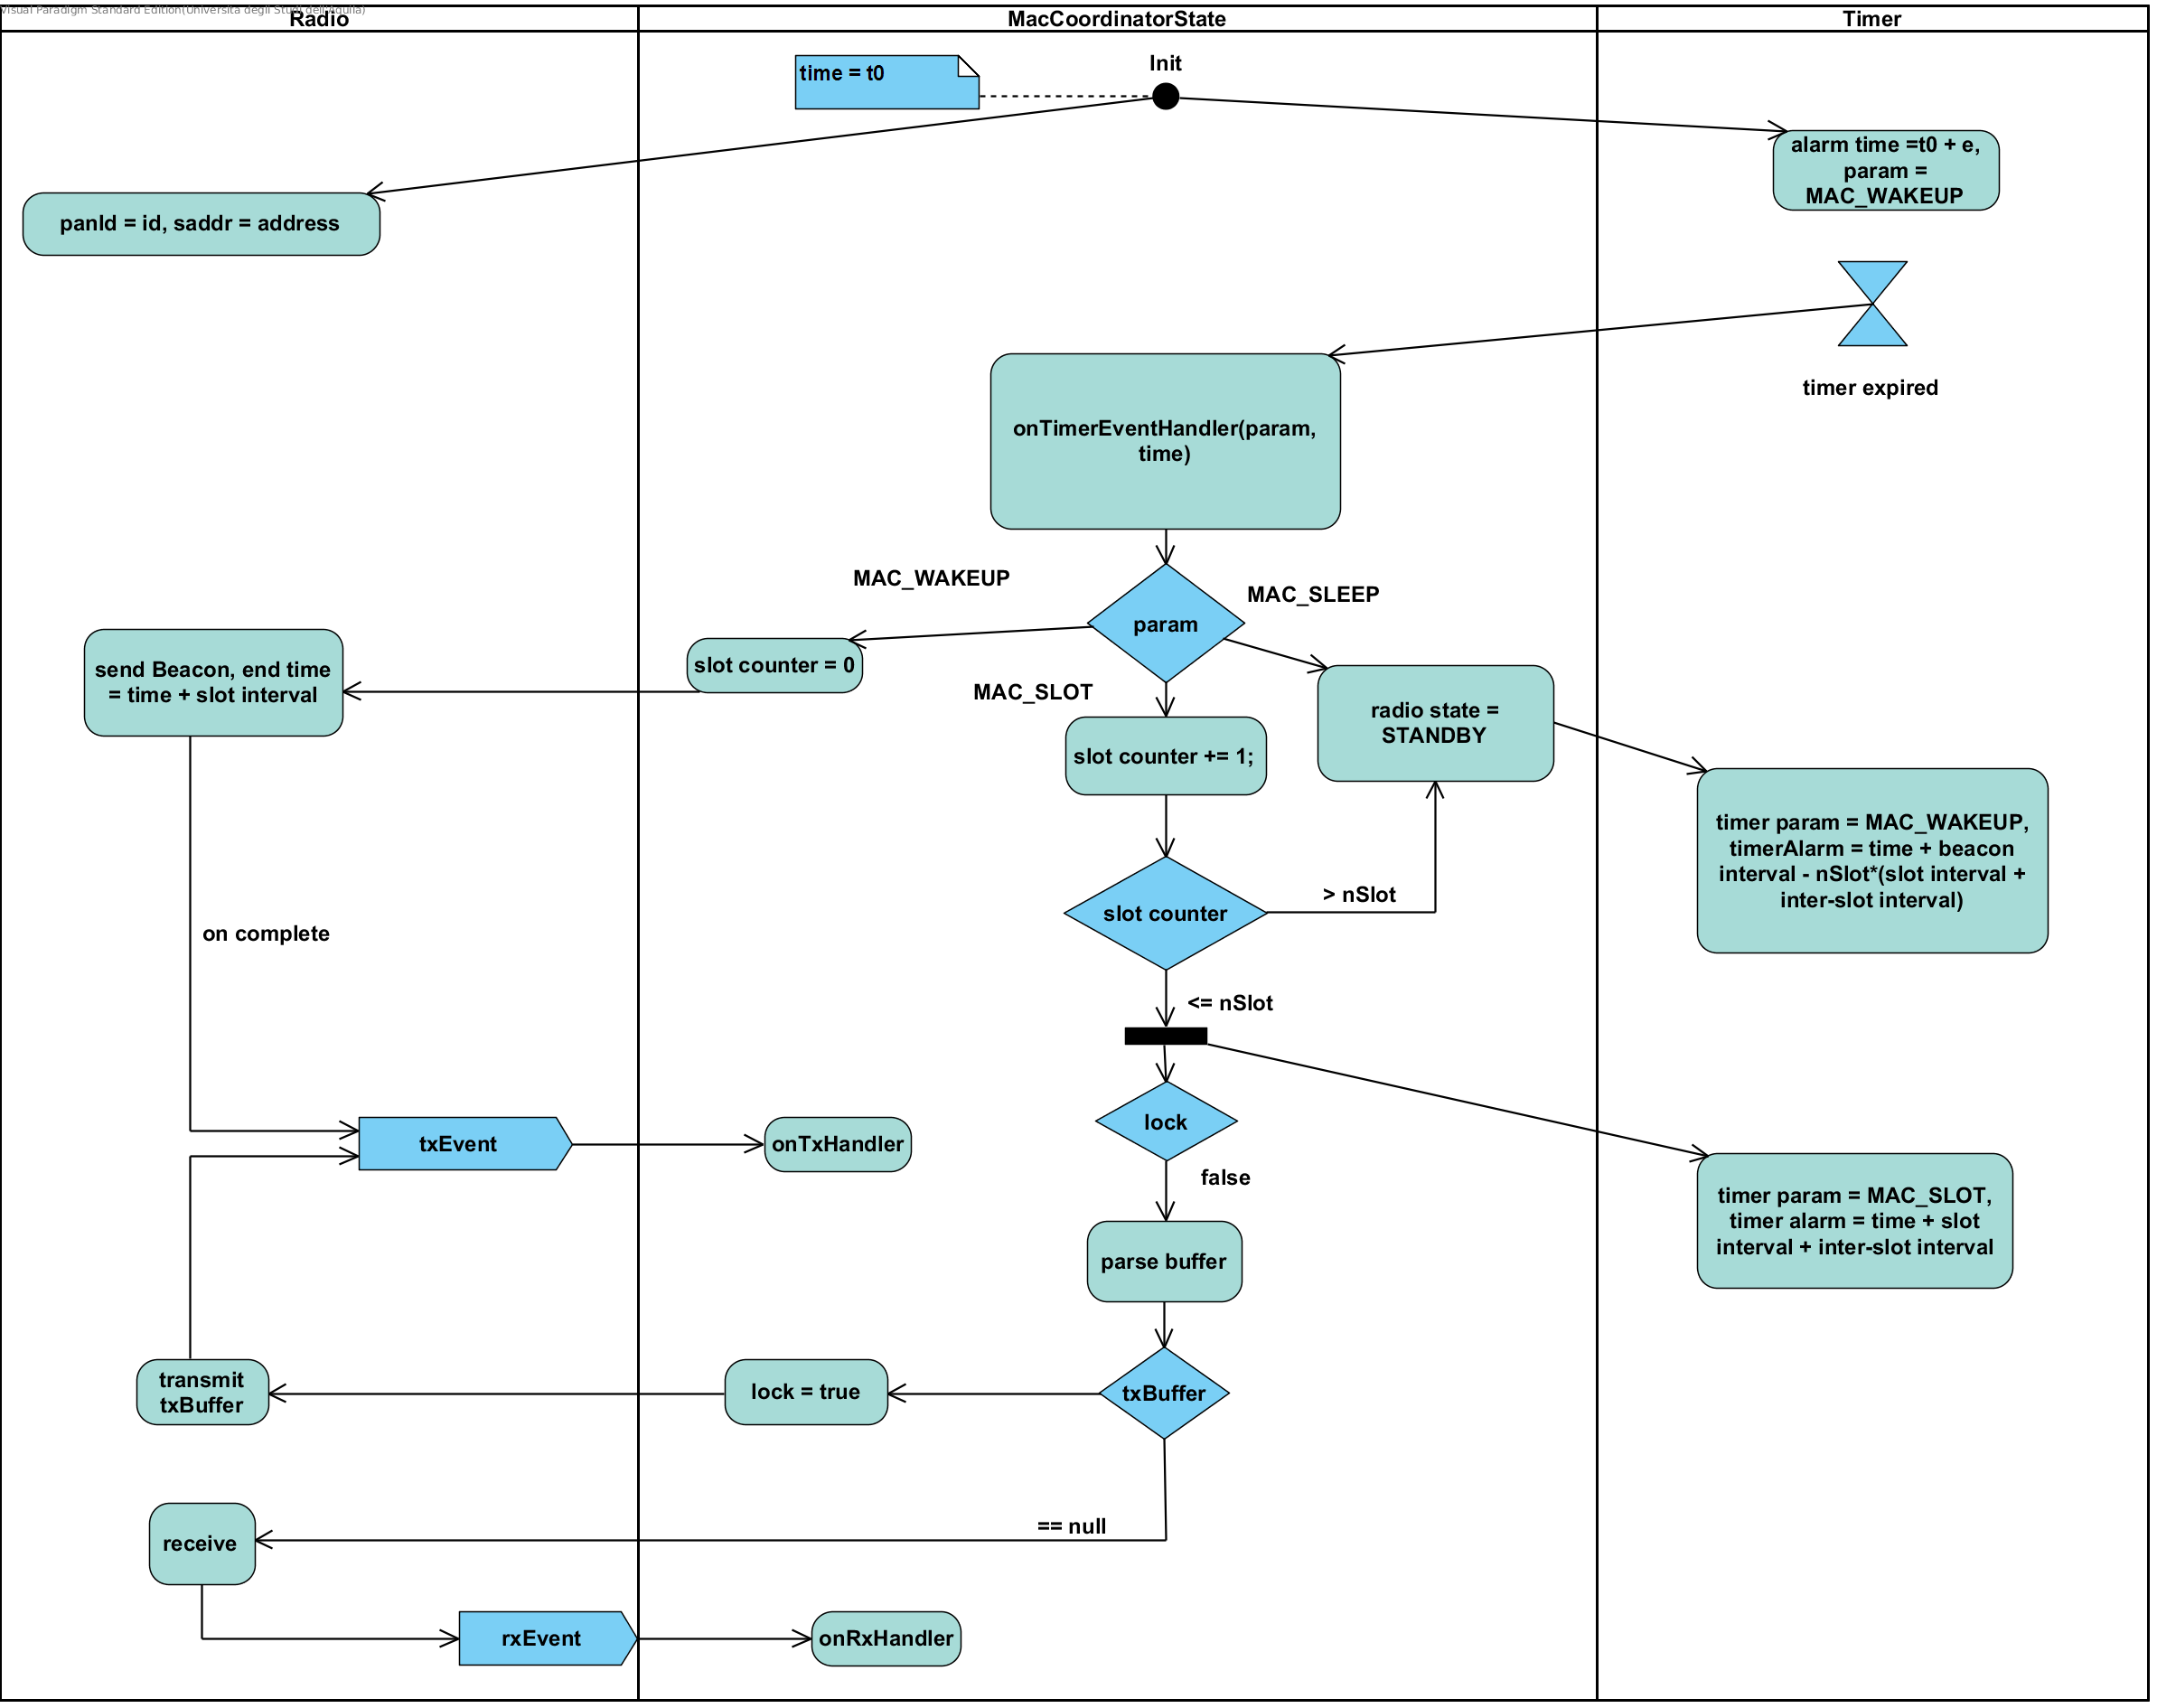
\includegraphics[width=.99\textwidth]{img/MAC_COORDINATOR.png}
  \end{figure}
\end{frame}

\begin{frame}[fragile]
  \frametitle{Example}
  \vspace{-2em}
  The node associates with coordinator, then responds to beacon pending list and gets data.
  \begin{figure}
    \centering
    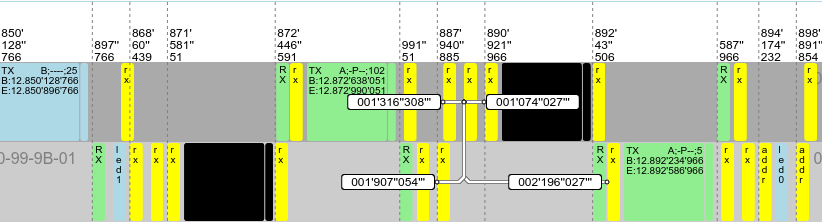
\includegraphics[width=\textwidth]{img/associazione.png}
  \end{figure}
  \begin{figure}
    \centering
    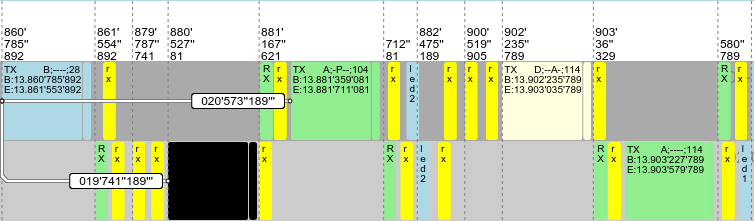
\includegraphics[width=\textwidth]{img/dataIndirect.png}
  \end{figure}
\end{frame}

\begin{frame}[fragile]
 \frametitle{Oscilloscope}
 \begin{columns}
    \begin{column}{.58\linewidth}
      \begin{itemize}
      	\item Periodically reads values of TEMPERATURE and LIGHT
      	\item Read interval and type can be setted by master
      	\item Readings are sent through MAC once associated to master
      	\item Readings done by MDA100 board
      \end{itemize}
    \end{column}
    \hfill
    \begin{column}{.4\linewidth}
      \begin{figure}
	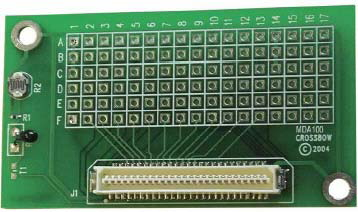
\includegraphics[width=\textwidth]{img/mda100.jpg}
      \end{figure}
    \end{column}
  \end{columns}
\end{frame}

\begin{frame}[fragile]
 \frametitle{Master Oscilloscope}
 \begin{columns}
    \begin{column}{.58\linewidth}
      \begin{itemize}
	\item It creates a PAN with the MAC layer
	\item It listens LIP for commands that sends to associated motes
	\item MAC layer sends readings to Master Oscilloscope that are redirected through LIP 
	\item A JavaScript Socket running on Sonoran process displays the readings
      \end{itemize}
  \end{column}
  \hfill
    \begin{column}{.4\linewidth}
      \begin{figure}
	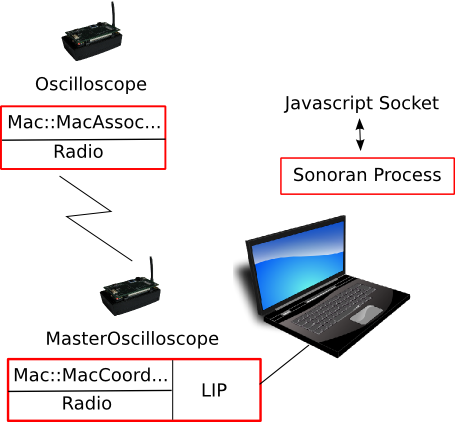
\includegraphics[width=\textwidth]{img/oscilloscope.png}
      \end{figure}
    \end{column}
  \end{columns}
\end{frame}

\begin{frame}[fragile]
	\frametitle{Live demo}
%	\begin{center}
%		\includemedia[activate=onclick,	width=0.75\textwidth]{\includegraphics{FK3.png}}{FK3.swf}
%	\end{center}	
\end{frame}